% !TEX root = owasp-doc.tex

% ================================================
%	LLM Strategy
% ================================================

\headerimage
\chapter{Determining LLM Strategy}
The rapid expansion of Large Language Model (LLM) applications has heightened
the attention and examination of all AI/ML systems used in business operations,
encompassing both Generative AI and long-established Predictive AI/ML systems.
This increased focus exposes potential risks, such as attackers targeting
systems that were previously overlooked and governance or legal challenges that
may have been disregarded in terms of legal, privacy, liability, or warranty
issues. For any organization leveraging AI/ML systems in its operations, it's
critical to assess and establish comprehensive policies, governance, security
protocols, privacy measures, and accountability standards to ensure these
technologies align with business processes securely and ethically.

Attackers, or adversaries, provide the most immediate and harmful threat to
enterprises, people, and government agencies. Their goals, which range from
financial gain to espionage, push them to steal critical information, disrupt
operations, and damage confidence. Furthermore, their ability to harness new
technologies such as AI and machine learning increases the speed and
sophistication of attacks, making it difficult for defenses to stay ahead of
attacks.

The most pressing non-adversary LLM threat for many organizations stem from
"Shadow AI": employees using unapproved online AI tools, unsafe browser
plugins, and third-party applications that introduce LLM features via updates
or upgrades, circumventing standard software approval processes.

\begin{figure}[h]
  \centering
  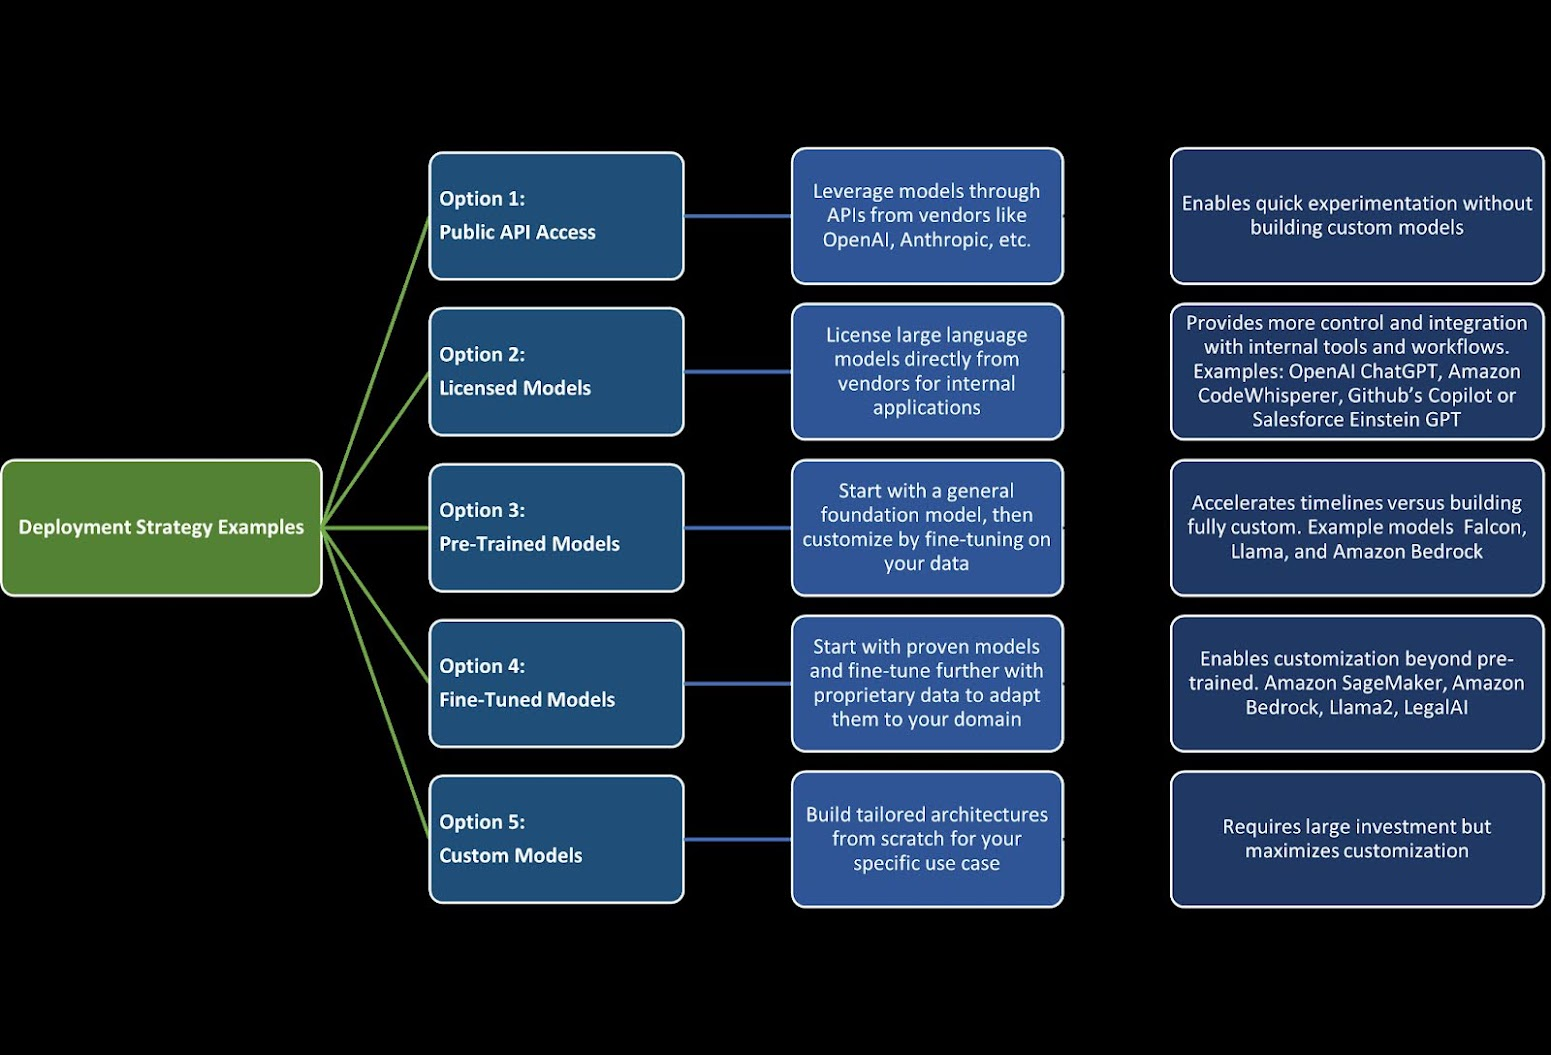
\includegraphics[width=\textwidth]{ai_deployment_strategy}
  \caption{Image of options for deployment strategy}
  \label{fig:llm-deployment-strategy}
\end{figure}

\clearpage

\section{Deployment Strategy}
The scopes range from leveraging public consumer applications to training
proprietary models on private data. Factors like use case sensitivity,
capabilities needed, and resources available help determine the right balance
of convenience vs. control. However, understanding these five model types
provides a framework for evaluating options.

\begin{figure}[h]
  \centering
  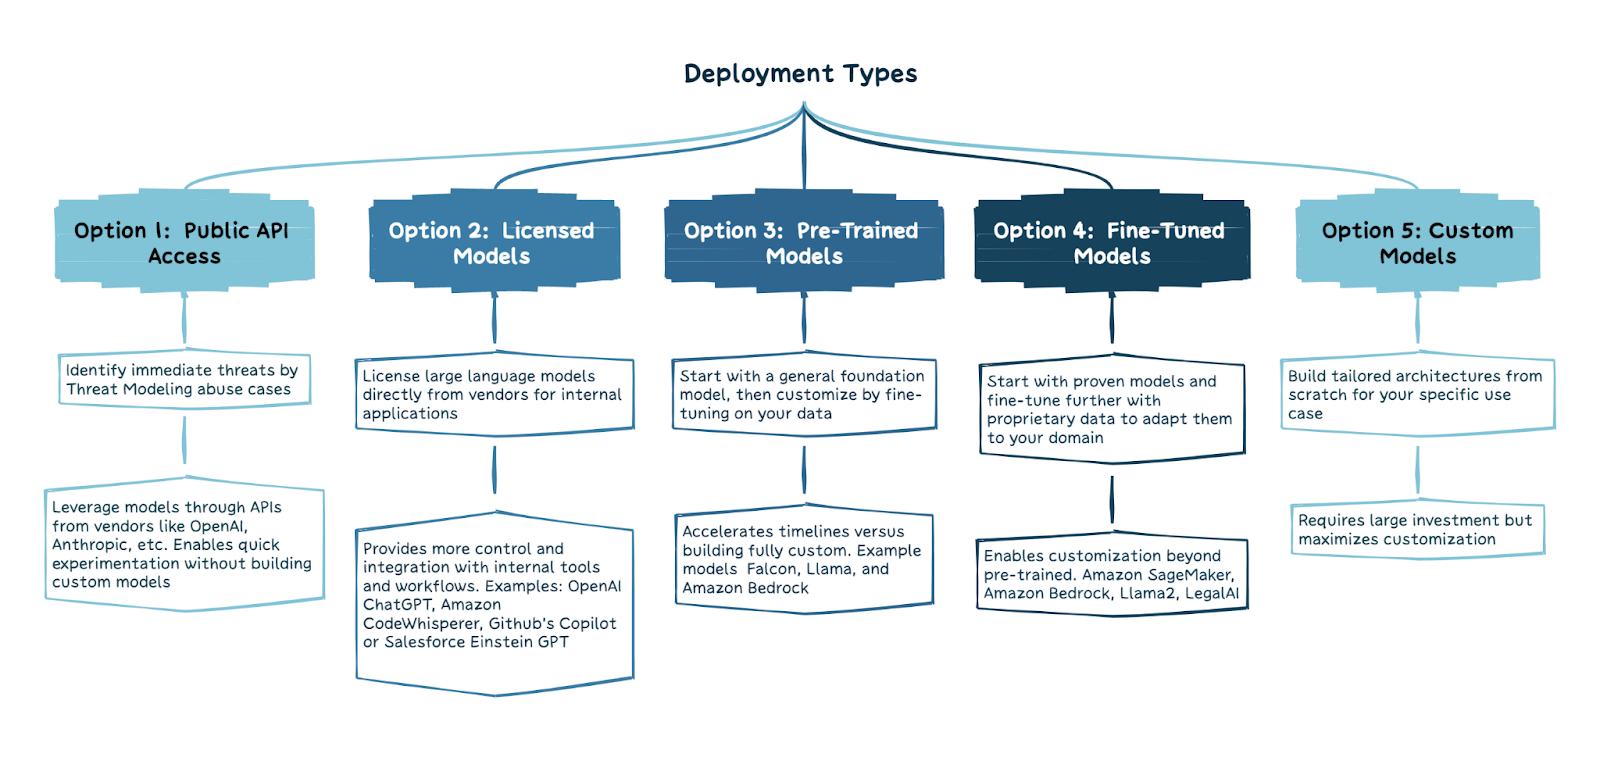
\includegraphics[width=\textwidth]{ai_deployment_types}
  \caption{Image of options for deployment types}
  \label{fig:llm-deployment-types}
\end{figure}
